% Define the document class:
\documentclass[12pt, a4paper, twoside]{article} % sometimes {report} might be better
% Set default font to sans serif
\renewcommand{\familydefault}{\sfdefault}
% Import any packages
\usepackage{graphicx} % for images
\usepackage{natbib}
\bibliographystyle{ctrH}
\usepackage{setspace}
\onehalfspacing
\usepackage[left=2cm, right=2cm, bottom=2.5cm, top=2cm]{geometry}
\usepackage{textcomp}
\usepackage{tabularx}
\usepackage{svg}

% Define Title and authors
\title{Executive Summary and Cloud Strategy for Retail Company Nugget \& Co.}
\author{Mark Collins \thanks{Nugget \& Co. is the trading name of Nugget \& Co. Jewellery Ltd, a real company of which the author has a vested interest.} \\ \textbf{Word Count:} 2107}
\date{\today}

\begin{document}
\maketitle

\section{Executive Summary}
Nugget \& Co. \citep{nugget2025} is an online, luxury gold jewellery retailer, aimed at middle-class and working women.  They are looking to deepen customer engagement, simplify operations, and scale internationally while preserving a premium brand experience. The business requires a cloud strategy that supports high-availability e-commerce, robust data analytics, personalised customer experiences, and strong security and conformance controls. Shopify Plus remains the e-commerce core for storefront and check-out \citep{aldea2018}, while Microsoft Azure provides the extensible cloud platform for integrations, data processing, AI-driven personalisation, and governance \citep{alkhatib2025, altemimi2022, perumal2025}. 

The proposed solution uses a hybrid SaaS-plus-cloud model:
\begin{itemize}
\item \textbf{Shpify Plus} handles transactional and storefront concerns.
\item \textbf{Azure} supplies:
	\begin{itemize}
	\item Serverless integration layers (API management, Function Apps), 
	\item Secure storage (Blob Storage), 
	\item Relational data (Azure SQL),
	\item Analytics (Azure Synapse \& Power BI)
	\item Machine learning (Azure ML)
	\end{itemize}
\item Infrastructure as Code (IaC) (\textbf{Terraform}) and CI/CD (\textbf{GitHub Actions}) automate provisioning and deployment, ensuring repeatable, auditable, and secure changes.
\item \textbf{Azure Active Directory} governs identity and access.
\item \textbf{Azure Policy} coupled with \textbf{Microsoft Defender} and \textbf{Sentinel} provides continuous security compliance monitoring.
\end{itemize}

Expected outcomes include improved site reliability during peak traffic, faster time-to-market for new features (AR try-on, personalised recommendations \citep{bialkova2022}), reduced operational overhead through managed pay-as-you-go services and serverless patterns, and clearer insights into customer behaviour that increases conversion and lifetime value. Risk mitigation and compliance controls reduce exposure to data breaches and regulatory fines, and the modular design positions Nugget \& Co. to adopt emerging technologies with minimal disruption. 

\section{Architecture Details}

\begin{figure}[h!]
 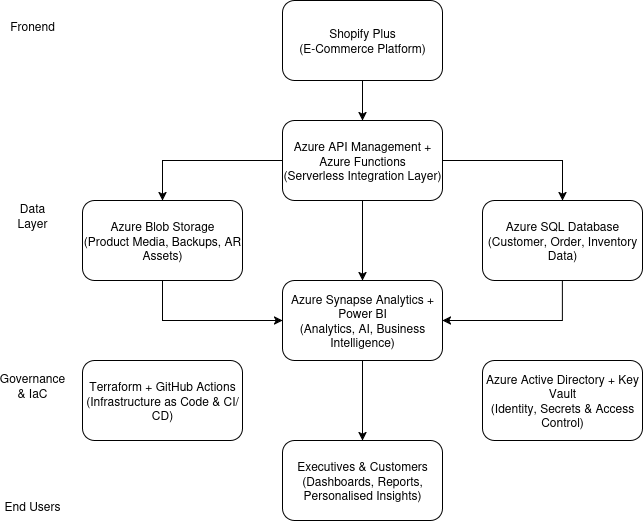
\includegraphics[width=\linewidth]{NuggetArch.png}
 \caption{Proposed Architecture for Nugget \& Co. using Shopify front end and Azure back end.}
 \label{fig:Arch}
\end{figure}

\begin{center}
\begin{tabularx}{1\textwidth}{
 | >{\raggedright\arraybackslash}X
 | >{\raggedright\arraybackslash}X
 | >{\raggedright\arraybackslash}X |
 }
\hline
\textbf{Function} & \textbf{Service} & \textbf{Benefit}\\
\hline \hline
\textbf{E-commerce} & Shopify Plus & Built-in PCI-DSS compliance. Provides support for start-up business, with room to grow.\\
\textbf{Integration Layer} & Azure API Management + Azure Functions & Securely connect Shopify Plus APIs to internal systems for inventory, shipping, and CRM updates.\\
\textbf{Data Storage} & Azure SQL Database \& Blob Storage & Reliable and scalable storage for order, product, and marketing data; supports Shopify exports and Power BI analytics.\\
\textbf{Analytics and AI} & Azure Synapse Analytics + Power BI & Enables cross-channel sales analytics, trend forecasting, and customer segmentation.\\
\textbf{Automation \& IaC} & Terraform on Azure + GitHub Actions & Infrastructure-as-Code ensures consistent, version-controlled deployments and lower operational risk.\\
\textbf{Security \& Identity} & Azure AD + Key Vault & Protects administrative access and customer data using enterprise-grade encryption and role-based access control.\\
\hline
\end{tabularx}
\end{center}


\section{Cloud Solution Design - Infrastructure as Code (IaC)}

The cloud solution for Nugget \& Co. is specified and deployed using Infrastructure as Code to ensure consistent, version-controlled infrastructure that supports scalability, security, and cost-effectiveness. 

\subsection{IaC Tooling \& Structure}
Terraform \citep{jayaram2024} is the recommended primary IaC tool due to its provider-agnostic approach, robust module ecosystem, and mature state management capabilities. The Terraform repository should be organised into reusable modules and environment overlays: 
\begin{itemize}
\item \texttt{modules/} (\texttt{vpc, storage, sql, function\_app, api\_management, monitoring, iam})
\item \texttt{envs/} (\texttt{dev, staging, prod}) with environment specific variables and work spaces
\item \texttt{global/backend.tf} configured for remote state in an Azure Storage Account with state locking (e.g. using Azure Blob Storage and lease-based locking strategies or Terraform Cloud)
\end{itemize}

GitHub Actions serves as the CI/CD engine \citep{decan2022}. Policies run at plan time (\texttt{tfsec, checkov}) to detect insecure configurations. Pull request workflows create a deterministic Terraform plan artefact and require code review and approval before apply to staging or production.


\subsection{Core Resource Design}
\begin{itemize}
\item \textbf{API Layer:} Azure API management fronts Azure Functions for webhook processing and lightweight microservices. Functions employ consumption or premium plans to autoscale with load. Each function is scoped with a dedicated manged identity and least-privilege role assignments.
\item \textbf{Storage:} Azure Blob Storage is the canonical store fir high-resolution media, AR models, and backups. Life cycle policies move older media to archive tiers and versioning protects against accidental deletion.
\item \textbf{Relational Data:} Azure SQL Database (single of Elastic Pod) stores customer profiles, inventory snapshots, and operational metadata not suitable for Shopify primary storage. Geo-replication is enabled for business continuity.
\item \textbf{Analytics:} Azure Synapse ingests event streams via Data Factory or Event Grid, with curated zones in Synapse Data Lake. Power BI connects to Synapse for dashboards and executive reporting.
\item \textbf{Observability:} Azure Monitor and Log Analytics collects metrics and logs. Alerts and action groups integrate with PagerDuty or Microsoft Teams for operational response. 
\item \textbf{Secrets \& Config:} Azure Key Vault centralises secrets, certificates, and connection strings; Terraform references Key Vault for non-checked-in sensitive values.
\item \textbf{Scalability:} The design uses serverless and managed services which scale automatically and keep costs aligned to usage. Azure Functions and API Management scale with concurrent connections, Blob Storage handles arbitrary volume, and Azure SQL can be configured with elastic pools or hyperscale to handle growth. IaC modules enable rapid provisioning of additional capacity or regions when expanding to new markets.
\item \textbf{Security:} Security is baked into the IaC approach \citep{verdet2025}. Terraform modules include guardrails: RBAC assignments, network rules (service endpoints and private endpoints for SQL and Storage), storage encryption, and logging configuration. Policy-as-code (Azure Policy) blocks public exposure of storage accounts, enforces required TLS versions, and mandates Key Vault use for secrets. Automated scanning pipelines (tfsec, checkov) prevent miss-configurations from reaching production.
\item \textbf{Cost Effectiveness:} Cost controls include lifecycle tiering for media, serverless compute to avoid idle costs, and reserved capacity for predictable analytics workloads. IaC enables automated environment scheduling (teardown or dev stacks) and tagging policies for charge back. Terraform-driven infra allows rapid identification and removal of unused resources.
\end{itemize}

\section{Integration of Advanced Cloud Technologies}
Nugget \& Co. will integrate advanced cloud technologies to deliver personalised customer experiences, automate operations, and adopt a hybrid approach where needed.
\subsubsection*{AI \& Machine Learning:}
Azure Machine Learning is the central service for training and deploying models. Typical use cases:
\begin{itemize}
\item \textit{Recommendation Engine:} Train collaborative filtering and content-based models on purchase and browsing data from Shopify and Synapse. Deploy as a managed endpoint or incorporate into Azure Functions for real-time recommendations.
\item \textit{Predictive Inventory:} Use time-series forcasting models to predict SKU replenishment needs and reduce stockouts for high-value pieces.
\item \textit{Customer Segmentation \& Customer Lifetime Value (CLV):} Use clustering and supervised models to identify high Lifetime Value (LTV) customers for targeted campaigns. 
\end{itemize}
Data pipelines use Azure Data Factory or Event Grid to stream Shopify events into Synapse, maintaining near-real-time capabilities. Models are versioned and reproducible through IaC and ML pipelines (Azure ML pipelines), ensuring consistent retraining and auditing.
\subsubsection*{Automation}
Robotic workflows and automation are applied to operational tasks:
\begin{itemize}
\item \textit{Order Enrichment:} Azure Functions automatically enrich orders with metadata and notify fulfilment systems.
\item \textit{Marketing Automation:} Triggered campaigns (abandoned cart, VIP alerts) use event-driven flows connecting Synapse insights to Klaviyo or HubSpot.
\item \textit{CI/CD for Apps \& Models:} GitHub Actions or Azure DevOps pipelines automate testing, container builds, and deployment of functions, Terraform changes, and ML artefacts \citep{decan2022}.
\end{itemize}
\subsubsection*{Hybrid Cloud Approach}
While Shopify Plus remains SaaS, a hybrid approach allows Nugget \& Co. to place sensitive or latency-critical workloads in an on-prem or Azure Edge setup if required. Azure Arc can extend governance to hybrid resources, ensuring consistent policy and security enforcement across cloud and on-prem infrastructure. Edge caching and CDN (Azure Front Door or Cloudflare) reduce latency for global customers. The Architecture supports vendor flexibility, with Terraform modules abstracting provider specifics. 

\pagebreak

\section{Risk and Compliance Considerations}

Risk assessment focuses on data protection, operational resilience, regulatory compliance and vendor dependencies.
\begin{center}
\begin{tabularx}{1.1\textwidth}{
 | >{\raggedright\arraybackslash}X
 | >{\raggedright\arraybackslash}X
 | >{\raggedright\arraybackslash}X |
 }
\hline
\textbf{Type} & \textbf{Risk} & \textbf{Mitigation} \\
\hline \hline
\textbf{Data Security \& Privacy} & Exposure of customer personal data and payment related information & Rely on Shopify Plus for payment processing (PCI-compliant). For supplemental data in Azure, enforce encryption at rest and in transit, private endpoints for databases, strict Key Vault usage and Data Loss Prevention (DLP) policies. Regularly run penetration tests and maintain an incident response plan. \\
\textbf{Operational Resilience} & Downtime during peak campaigns or outages affecting API integrations & Use retry patterns, idempotent webhook handlers and queuing (Azure Service Bus) to decouple systems. Implement health checks, autoscale rules, and cross-region fail over for critical storage and databases. \\
\textbf{Regulatory Compliance} & GDPR, CCPA, and regional data residency requirements & Maintain data mapping and processing records. Use Synapse and Blob Storage with region choice aligned to residency constraints. Implement data retention policies and subject access request workflows. Use Azure Policy and Blueprints to ensure resources are provisioned in compliant ways. \\
\textbf{Vendor \& Supply Chain Risks} & Dependency on third-party services (Shopify apps, connectors) & Evaluate third-party SLA's, maintain minimal critical-path reliance, and prefer open standards for integrations. Use abstraction layer (API Management) to swap providers with minimal changes. \\
\hline
\end{tabularx}
\end{center}

\subsection{Governance and Controls}
Actionable steps:
\begin{enumerate}
\item Implement a security baseline with Azure Security Centre and Sentinel for SIEM capabilities \citep{praveenborra2024}.
\item Use Policy-as-code to block insecure resources and require monitoring \citep{chuprikov2025a}.
\item Schedule audit and compliance reviews with external auditors annually.
\item Maintain runbooks and disaster recovery drills, including simulated fail-overs \citep{gupta2024}.
\end{enumerate}

\section{Future Recommendations}

To ensure long-term competitiveness and technical agility, Nugget\& Co. should consider the following forward looking initiatives:
\subsubsection*{Edge Computing}
Leverage Azure Front Door and Azure CDN to cache product media and AR assets at the edge, reducing latency for global customers. Evaluate Azure IoT Edge or Azure Stack if in-person experiences require low-latency processing (e.g. in-store AR mirrors) \citep{borra2024a}.
\subsubsection*{Composable Commerce}
Gradually implement headless storefront elements where performance or customisation demands exceed Shopify theme capabilities. Use Shopify Storefront API combined with Azure-hosted front end components for selective headless experiences.
\subsubsection*{Generative AI for Content}
Use Azure OpenAI to generate product descriptions, marketing copy, and creative A/B tests. Ensure human-in-the-loop review for brand voice and regulatory accuracy.
\subsubsection*{Quantum-Ready Planning}
Monitor quantum-safe encryption standards and maintain crypto-agility in key management. While quantum cloud adoption is premature, design key rotation and algorithm migration plans.
\subsubsection*{Sustainability}
Track carbon footprint of cloud usage via Azure sustainability tools and preferentially use regions with lower carbon intensity. Pilot programs with defined KPI's (conversion uplift, latency reduction, cost per acquisition) are recommended to validate impact before wider rollout.

\section{Roadmap}

\subsection*{Phase 1: Discovery and Planning}
\begin{itemize}
\item \textbf{Business Assessment:} Review Shopify workflows, sales channels, and back-end systems (CRM, inventory, fulfillment).
\item \textbf{Technical Audit:} Assess current hosting, data exports, and existing automations.
\item \textbf{Architecture Blueprinting:} Define high-level Azure architecture.
\item \textbf{IaC \& DevOps Standards:} Select Terraform structure, define GitHub Actions CI/CD pipeline.
\item \textbf{Compliance Review:} Map GDPR, PCI DSS, and data residency requirements.
\end{itemize}

\subsection*{Phase 2: Foundation Build}
\begin{itemize}
\item \textbf{Infrastructure Deployment:} Create VNET, subnets, storage accounts, SQL DB, and Functions App using Terraform modules.
\item \textbf{Identity \& Access:} Configure Azure Active Directory roles, MFA, and Key Vault secrets.
\item \textbf{Networking \& Security:} Implement NSGs, private endpoints, and initial monitoring with Azure Monitor.
\item \textbf{CI/CD Setup:} Configure GitHub Actions for automated Terraform plan/apply.
\item \textbf{Environment Provisioning:} Create \texttt{dev}, \texttt{test}, and \texttt{prod} resource groups.
\end{itemize}

\subsection*{Phase 3: Integration \& Data Enablement}
\begin{itemize}
\item \textbf{API Integration:} Develop Functions to synchronise Shopify data (orders, products, customers).
\item \textbf{Data Storage \& ETL:} Establish pipelines from Shopify exports $\rightarrow$ Blob Storage $\rightarrow$ SQL Database.
\item \textbf{Monitoring \& Logging:} Implement Application Insights for Function Apps.
\item \textbf{Analytics Layer Setup:} Deploy Azure Synapse workspace and initial Power BI dashboards.
\item \textbf{Governance Automation:} Enforce Azure Policy for tagging, encryption, and cost tracking.
\end{itemize}

\subsection*{Phase 4: AI, Automation \& Advanced Analytics}
\begin{itemize}
\item \textbf{AI \& ML Enablement:} Use Azure Machine Learning for predictive models (demand forecasting, customer clustering).
\item \textbf{Recommendation Engine:} Integrate Azure Cognitive Services for product recommendations).
\item \textbf{Power BI Enhancement:} Create interactive, automated dashboards for executives.
\item \textbf{Process Automation:} Implement Logic Apps for workflow automation (inventory alerts, fulfilment notifications).
\item \textbf{Security Review:} Conduct penetration testing and threat modelling before production go-live.
\end{itemize}

\subsection*{Phase 5: Production Deployment \& Optimisation}
\begin{itemize}
\item \textbf{Production Rollout:} Deploy all infrastructure and pipelines to production environments.
\item \textbf{Load \& Stress Testing:} Validate scalability for peak sales (e.g. seasonal promotions).
\item \textbf{Cost Optimisation:} Apply reserved capacity, right-size resources, enable budgets.
\item \textbf{Disaster Recovery Setup:} Configure geo-redundant backups and restore simulations.
\item \textbf{Training \& Handover:} Train internal IT and business teams on monitoring and usage.
\end{itemize}

\subsection*{Phase 6: Continuous Improvement \& Future Readiness}
\begin{itemize}
\item \textbf{Operational Excellence:} Regular reviews of usage, security, and cost efficiency.
\item \textbf{AI Model Expansion:} Extent ML models for customer lifetime value, churn prediction.
\item \textbf{Edge Computing Exploration:} Pilot AR enabled in-person experiences powered by Azure Edge.
\item \textbf{Sustainability Metrics:} Integrate Azure Sustainability Manager to monitor carbon impact.
\item \textbf{Innovation Pipeline:} Engage with Azure Quantum or partner AI labs for R\&D initiatives. 
\end{itemize}

\section{Conclusion}
Nugget \& Co.'s adoption of a Shopify Plus core augmented by a well-architected Azure platform, deployed via Infrastructure as Code, provides an optimal balance between brand experience, operational control, and future agility. The proposed architecture and controls enable high availability, data-driven personalisation, and secure operations while keeping costs aligned with demand through serverless and managed services. By following the described IaC practices, integrating AI and automation responsibly, and addressing risks through policy and tooling Nugget \& Co. will be well-positioned to scale its digital presence and innovate confidently in the luxury jewellery market.

\bibliography{./COM}

\end{document}
